\documentclass[
  shownotes,
  xcolor={svgnames},
  hyperref={colorlinks,citecolor=DarkBlue,linkcolor=andesred,urlcolor=DarkBlue}
  , aspectratio=169]{beamer}
\usepackage{animate}
\usepackage{amsmath}
\usepackage{amsfonts}
\usepackage{amssymb}
\usepackage{pifont}
\usepackage{mathpazo}
%\usepackage{xcolor}
\usepackage{multimedia}
\usepackage{fancybox}
\usepackage[para]{threeparttable}
\usepackage{multirow}
\setcounter{MaxMatrixCols}{30}
\usepackage{subcaption}
\usepackage{graphicx}
\usepackage{lscape}
\usepackage[compatibility=false,font=small]{caption}
\usepackage{booktabs}
\usepackage{ragged2e}
\usepackage{chronosys}
\usepackage{appendixnumberbeamer}
\usepackage{animate}
\setbeamertemplate{caption}[numbered]
\usepackage{color}
%\usepackage{times}
\usepackage{tikz}
\usepackage{comment} %to comment
%% BibTeX settings
\usepackage{natbib}
\bibliographystyle{apalike}
\bibpunct{(}{)}{,}{a}{,}{,}
\setbeamertemplate{bibliography item}{[\theenumiv]}

% Defines columns for bespoke tables
\usepackage{array}
\newcolumntype{L}[1]{>{\raggedright\let\newline\\\arraybackslash\hspace{0pt}}m{#1}}
\newcolumntype{C}[1]{>{\centering\let\newline\\\arraybackslash\hspace{0pt}}m{#1}}
\newcolumntype{R}[1]{>{\raggedleft\let\newline\\\arraybackslash\hspace{0pt}}m{#1}}


\usepackage{xfrac}


\usepackage{multicol}
\setlength{\columnsep}{0.5cm}

% Theme and colors
\usetheme{Boadilla}

% I define a custom pallete
\definecolor{andesred}{HTML}{1B175E}
\definecolor{andesyellow}{HTML}{ffff00}

% Other options
\providecommand{\U}[1]{\protect\rule{.1in}{.1in}}
\usefonttheme{serif}
\setbeamertemplate{itemize items}[default]
\setbeamertemplate{enumerate items}[square]
\setbeamertemplate{section in toc}[circle]


\definecolor{mybackground}{HTML}{1B175E}
\definecolor{myforeground}{HTML}{0000A0}

\setbeamercolor{normal text}{fg=black,bg=white}
\setbeamercolor{alerted text}{fg=andesred}
\setbeamercolor{example text}{fg=black}

\setbeamercolor{background canvas}{fg=myforeground, bg=white}
\setbeamercolor{background}{fg=myforeground, bg=mybackground}
\setbeamercolor{palette tertiary}{fg=myforeground,bg=mybackground}

\setbeamercolor{palette primary}{fg=black, bg=white}
\setbeamercolor{palette secondary}{fg=black, bg=white!10!andesyellow}
\setbeamercolor{palette tertiary}{fg=black, bg=white}


\setbeamercolor{frametitle}{fg=black}
\setbeamercolor{title}{fg=black}
\setbeamercolor{block title}{fg=andesred}
\setbeamercolor{itemize item}{fg=andesred}
\setbeamercolor{itemize subitem}{fg=andesred}
\setbeamercolor{itemize subsubitem}{fg=andesred}
\setbeamercolor{enumerate item}{fg=andesred}
\setbeamercolor{item projected}{bg=gray!30!white,fg=andesred}
\setbeamercolor{enumerate subitem}{fg=andesred}
\setbeamercolor{section number projected}{bg=gray!30!white,fg=andesred}
\setbeamercolor{section in toc}{fg=andesred}
\setbeamercolor{caption name}{fg=andesred}
\setbeamercolor{button}{bg=gray!30!white,fg=andesred}
\setbeamercolor{title in head/foot}{fg=andesred}



\usepackage{fancyvrb}
\newcommand{\VerbBar}{|}
\newcommand{\VERB}{\Verb[commandchars=\\\{\}]}
\DefineVerbatimEnvironment{Highlighting}{Verbatim}{commandchars=\\\{\}}
% Add ',fontsize=\small' for more characters per line
\usepackage{framed}
\definecolor{shadecolor}{RGB}{248,248,248}
\newenvironment{Shaded}{\begin{snugshade}}{\end{snugshade}}
\newcommand{\AlertTok}[1]{\textcolor[rgb]{0.94,0.16,0.16}{#1}}
\newcommand{\AnnotationTok}[1]{\textcolor[rgb]{0.56,0.35,0.01}{\textbf{\textit{#1}}}}
\newcommand{\AttributeTok}[1]{\textcolor[rgb]{0.77,0.63,0.00}{#1}}
\newcommand{\BaseNTok}[1]{\textcolor[rgb]{0.00,0.00,0.81}{#1}}
\newcommand{\BuiltInTok}[1]{#1}
\newcommand{\CharTok}[1]{\textcolor[rgb]{0.31,0.60,0.02}{#1}}
\newcommand{\CommentTok}[1]{\textcolor[rgb]{0.56,0.35,0.01}{\textit{#1}}}
\newcommand{\CommentVarTok}[1]{\textcolor[rgb]{0.56,0.35,0.01}{\textbf{\textit{#1}}}}
\newcommand{\ConstantTok}[1]{\textcolor[rgb]{0.00,0.00,0.00}{#1}}
\newcommand{\ControlFlowTok}[1]{\textcolor[rgb]{0.13,0.29,0.53}{\textbf{#1}}}
\newcommand{\DataTypeTok}[1]{\textcolor[rgb]{0.13,0.29,0.53}{#1}}
\newcommand{\DecValTok}[1]{\textcolor[rgb]{0.00,0.00,0.81}{#1}}
\newcommand{\DocumentationTok}[1]{\textcolor[rgb]{0.56,0.35,0.01}{\textbf{\textit{#1}}}}
\newcommand{\ErrorTok}[1]{\textcolor[rgb]{0.64,0.00,0.00}{\textbf{#1}}}
\newcommand{\ExtensionTok}[1]{#1}
\newcommand{\FloatTok}[1]{\textcolor[rgb]{0.00,0.00,0.81}{#1}}
\newcommand{\FunctionTok}[1]{\textcolor[rgb]{0.00,0.00,0.00}{#1}}
\newcommand{\ImportTok}[1]{#1}
\newcommand{\InformationTok}[1]{\textcolor[rgb]{0.56,0.35,0.01}{\textbf{\textit{#1}}}}
\newcommand{\KeywordTok}[1]{\textcolor[rgb]{0.13,0.29,0.53}{\textbf{#1}}}
\newcommand{\NormalTok}[1]{#1}
\newcommand{\OperatorTok}[1]{\textcolor[rgb]{0.81,0.36,0.00}{\textbf{#1}}}
\newcommand{\OtherTok}[1]{\textcolor[rgb]{0.56,0.35,0.01}{#1}}
\newcommand{\PreprocessorTok}[1]{\textcolor[rgb]{0.56,0.35,0.01}{\textit{#1}}}
\newcommand{\RegionMarkerTok}[1]{#1}
\newcommand{\SpecialCharTok}[1]{\textcolor[rgb]{0.00,0.00,0.00}{#1}}
\newcommand{\SpecialStringTok}[1]{\textcolor[rgb]{0.31,0.60,0.02}{#1}}
\newcommand{\StringTok}[1]{\textcolor[rgb]{0.31,0.60,0.02}{#1}}
\newcommand{\VariableTok}[1]{\textcolor[rgb]{0.00,0.00,0.00}{#1}}
\newcommand{\VerbatimStringTok}[1]{\textcolor[rgb]{0.31,0.60,0.02}{#1}}
\newcommand{\WarningTok}[1]{\textcolor[rgb]{0.56,0.35,0.01}{\textbf{\textit{#1}}}}
\usepackage{graphicx}
\makeatletter

\makeatother






%%%%%%%%%%%%%%% BEGINS DOCUMENT %%%%%%%%%%%%%%%%%%

\AtBeginSection[]
{
    \begin{frame}
        \frametitle{Agenda}
        \tableofcontents[currentsection]
    \end{frame}
}

\begin{document}

\title{Prediction and Linear Regression}
\subtitle{Big Data y Machine Learning para Economía Aplicada}
\date{}

\author[Sarmiento-Barbieri]{Ignacio Sarmiento-Barbieri}
\institute[Uniandes]{Universidad de los Andes}


\begin{frame}[noframenumbering]
\maketitle
\end{frame}

%%%%%%%%%%%%%%%%%%%%%%%%%%%%%%%%%%%
%       Motivation              %
% What is the question?
% Why do we care?
% What is new?
% What do you find?
%%%%%%%%%%%%%%%%%%%%%%%%%%%%%%%%%%%




\begin{frame}
\frametitle{Agenda}

\tableofcontents


\end{frame}




%----------------------------------------------------------------------%
%----------------------------------------------------------------------%
\section{Prediction and loss functions}
%----------------------------------------------------------------------%
%----------------------------------------------------------------------%
%----------------------------------------------------------------------%
\begin{frame}
\frametitle{Getting serious about prediction}


\begin{align}
y=f(X)+u
\end{align}

\begin{itemize}
  \item Interest on predicting $Y$
  \medskip
  \item Model? We  treat $f()$ as a black box, and any approximation $\hat{f}()$ that yields a good prediction is good enough ({\it ``Whatever works, works...''}).
  \medskip
  \item How do we measure ``what works''?
  \pause
  \medskip
  \item Formal statistics can help  figure out this: what is a good prediction.

\end{itemize}


\end{frame}
%----------------------------------------------------------------------%
\begin{frame}
\frametitle{Minimizing our losses}
\begin{itemize}
\item A very common loss function in a regression setting is the squared loss $L(d)=d^2$
\medskip
\item Under this loss function the expected prediction loss  is the mean squared error (MSE)
\medskip
  

\item {\bf Result}: The best prediction of $Y$ at any point $X = x$ is the conditional mean, when best is measured using a square error loss
\end{itemize}


\end{frame}
%----------------------------------------------------------------------%
\begin{frame}
\frametitle{Minimizing our losses}

\begin{itemize}
\item Prediction problem solved if we knew $f^* = E[y|X=x]$ 
\pause
\medskip
\item But we have to settle for an estimate: $\hat{f}(x)$
\medskip
\item The EMSE of this

\begin{align}
E(y-\hat y)^2 &= E(f(X)+u - \hat f(X))^2 
\end{align}
\end{itemize}

\end{frame}

%----------------------------------------------------------------------%
\begin{frame}
\frametitle{Reducible and irreducible error}

\begin{align}
E(y-\hat y)^2  &= \underset{Reducible}{\underbrace{[f(X)-\hat{f}(X)]^{2}}}+\underset{Irreducible}{\underbrace{Var(u)}}
\end{align}
\bigskip
\begin{itemize}
\item The focus the is on techniques for estimating $f$ with the aim of minimizing the reducible error
\medskip
\item It is important to keep in mind that the irreducible error will always provide an upper bound on the accuracy of our prediction for $y$
\medskip
\item This bound is almost always unknown in practice
\end{itemize}


\end{frame}
%----------------------------------------------------------------------%

\begin{frame}<1>[label=bias_variance]
\frametitle{Bias/Variance Decomposition}

Recall that 
\begin{itemize}
  \item $Bias (\hat f(X) )=E (\hat f(X) )-f=E (\hat f(X)-f(X))$
  \item  $Var (\hat f(X))  =E (\hat f(X) - E (\hat f(X)))^2$
\end{itemize}
\pause
\bigskip
{\bf Result} (very important!)
\bigskip

\begin{align}
  EMSE = Bias^2 (\hat f(X))+V (\hat f(X)) +\underset{Irreducible}{\underbrace{Var(u)}}
\end{align}

{\tiny HW: Proof}

\end{frame}


%----------------------------------------------------------------------%
\begin{frame}
\frametitle{Bias/Variance Decomposition}

\begin{figure}[H] \centering
  \centering
  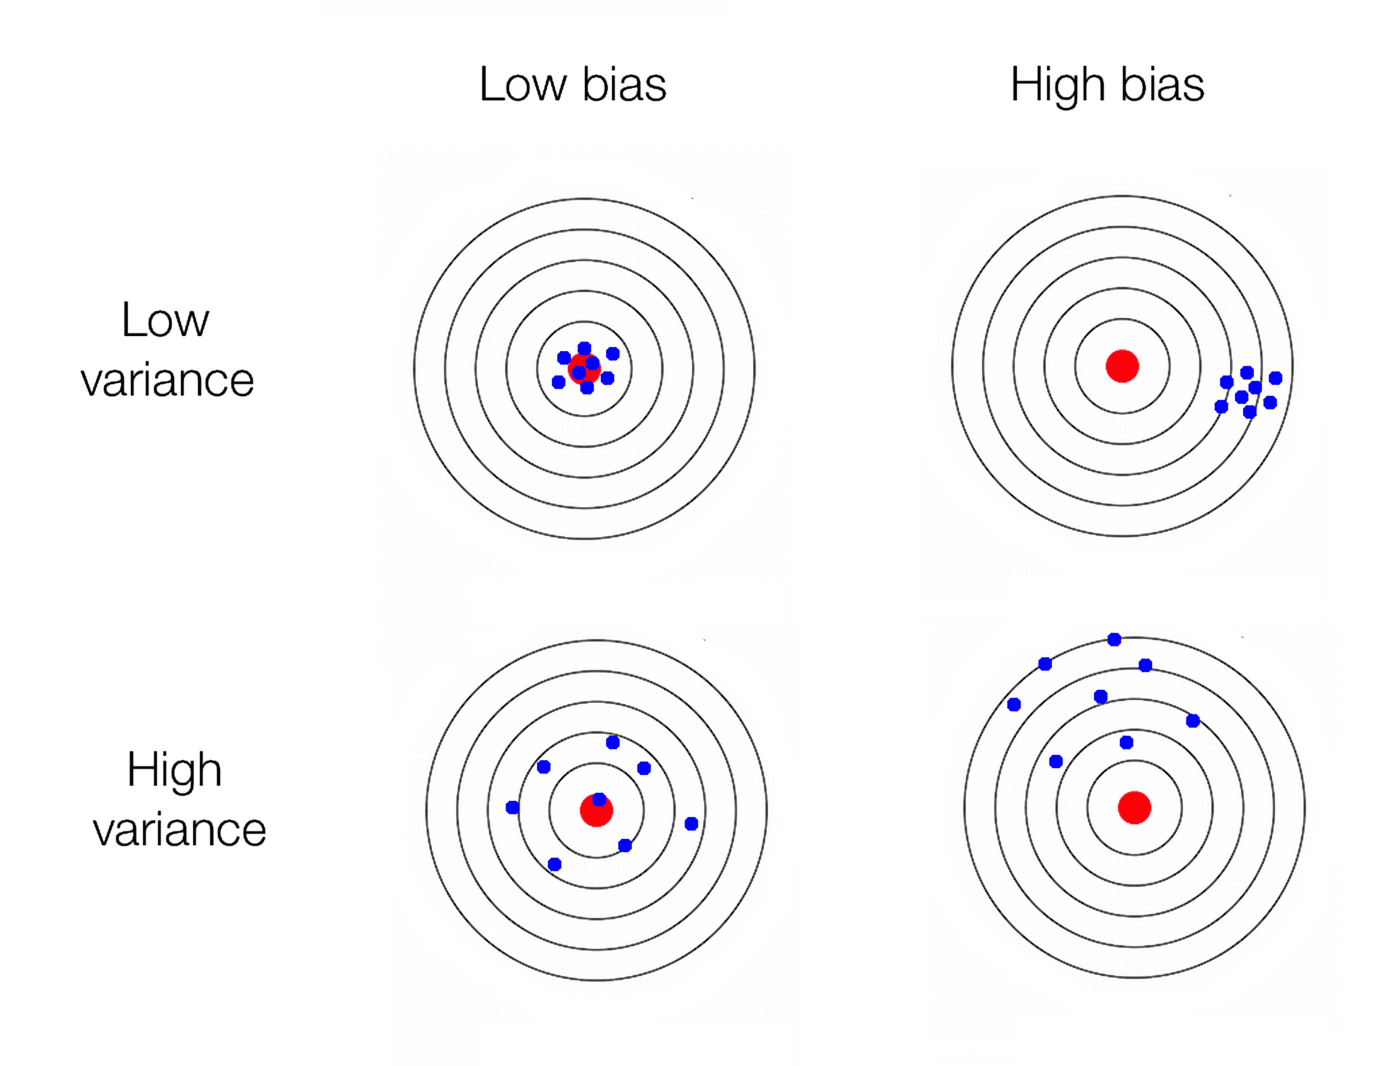
\includegraphics[scale=0.15]{figures/medium_bias_variance}
  \\
  \tiny
  Source: https://tinyurl.com/y4lvjxpc
\end{figure}

\end{frame}


%----------------------------------------------------------------------%
%----------------------------------------------------------------------%
\againframe<2>{bias_variance}
%----------------------------------------------------------------------%
%----------------------------------------------------------------------%

%----------------------------------------------------------------------%
\begin{frame}
\frametitle{Bias/Variance Decomposition}



\begin{minipage}[t]{0.45\linewidth}
        \begin{figure}[H] \centering
            \captionsetup{justification=centering}  
            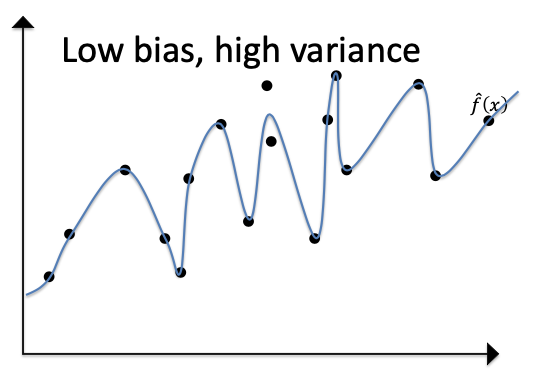
\includegraphics[scale=0.65]{figures/low_bias_high_variance.png}
            
    \end{figure}
    \end{minipage}
    \hfill
    \begin{minipage}[t]{0.45\linewidth}%
        \begin{figure}[H] \centering
            \captionsetup{justification=centering}  
            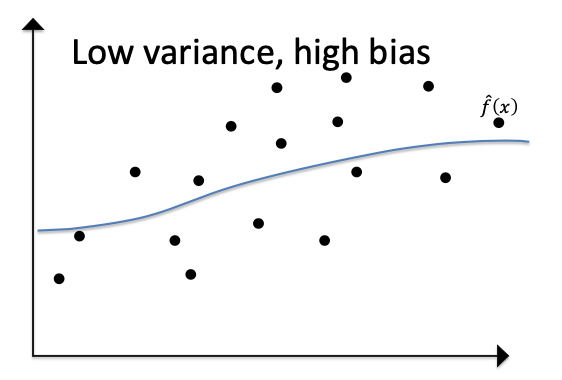
\includegraphics[scale=0.65]{figures/high_bias_low_variance.png}
            
    \end{figure}
    \end{minipage}


\end{frame}

%----------------------------------------------------------------------%

\begin{frame}
\frametitle{The Bias-Variance Trade-Off}

\begin{align}
  EMSE = Bias^2 (\hat f(X))+V (\hat f(X)) +\underset{Irreducible}{\underbrace{Var(u)}}
\end{align}



\begin{figure}[H] \centering
  \centering
  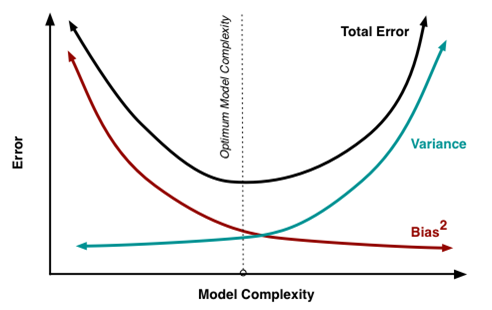
\includegraphics[scale=0.35]{figures/medium_bias_variance_trade_off.png}
  \\
  \tiny
  Source: https://tinyurl.com/y4lvjxpc
\end{figure}
\begin{itemize}
  
  \item The best kept secret: tolerating some bias is possible to reduce V($\hat f(X)$) and lower MSE
  
\end{itemize}
\end{frame}




%----------------------------------------------------------------------%
\begin{frame}
\frametitle{Prediction and linear regression}




\begin{itemize}
  \item The goal is to predict $y$ given another variables $X$. 
  \medskip
  \item We  assume that the link between $y$ and $X$ is given by the simple model:


\begin{align}
  y = f(X) + u
\end{align}

\item we just learned that under a squared loss we need to approximate $E[y|X=x]$
\end{itemize}

\end{frame}
%----------------------------------------------------------------------%
\begin{frame}
\frametitle{Prediction and linear regression}

\begin{itemize}
\item As economists we know that we can approximate $E[y|X=x]$ with a linear regression

\begin{align}
  f(X) = \beta_0 + \beta_1 X_1 + \dots + \beta_p X_p 
\end{align}

\item The problem boils down to estimating $\beta$s
\medskip
\item We can estimate these using
  \begin{itemize}
    \footnotesize
    \item  OLS
    \medskip
    \item MLE
    \medskip
    \item MM
  \end{itemize}  
\end{itemize}

\end{frame}
%----------------------------------------------------------------------%
\begin{frame}

\begin{figure}[H] \centering
  \centering
  
\includegraphics[scale=0.35]{figures/baticomputer_meme.jpg}
  \\
  \tiny photo from \url{https://www.dailydot.com/parsec/batman-1966-labels-tumblr-twitter-vine/}
\end{figure}

\end{frame}
%----------------------------------------------------------------------%
\begin{frame}
\frametitle{Prediction and linear regression}

\begin{itemize}
  \item And the Bias-Variance Trade-Off?
  \pause
  \item Under the classical assumptions the OLS estimator is unbiased, hence 

\medskip
\begin{align}
  E( X \hat \beta)&= E(\hat{\beta}_1 + \hat{\beta}_2 X_2 + \dots + \hat{\beta}_p X_p) \\ 
  &= E(\hat{\beta}_1) + E(\hat{\beta}_2) X_2 + \dots + E(\hat{\beta}_p) X_p  \\ 
  &= X \beta
\end{align}
\medskip




\item Then, 

\begin{itemize}
  \item $MSE(\hat f)$ reduces to just $V(\hat f)$
\end{itemize} 



\end{itemize}

\end{frame}


%----------------------------------------------------------------------%
\begin{frame}
\frametitle{Complexity and the variance/bias trade off}

\begin{itemize}

  \item When the focus switches from estimating $f$ to predicting $Y$, 
  \medskip
  \item $f$ plays a secondary role, as just a tool to improve the prediction based on $X$.
  \medskip
  \item  Predicting $Y$ involves \emph{learning} $f$, that is, $f$ is no longer taken as given, as in the classical view. 
  \medskip
  \item Now it implies an iterative process where initial choices for $f$ are revised in light of potential improvements in predictive performance.
  \medskip
  \item Model choice or learning involves choosing both $f$ and a strategy to estimate it ($\hat f$), guided by predictive performance. 

\end{itemize}


\end{frame}
%----------------------------------------------------------------------%
\begin{frame}
\frametitle{Complexity and the variance/bias trade off}

\begin{itemize}
\item Classical econometrics, model choice involves deciding between a smaller and a larger linear model. 

\item Consider the following competing models for $y$:

\end{itemize}



\begin{minipage}[t]{0.48\linewidth}

          \begin{equation} 
          y=\beta_1 X_1 + u_1 \nonumber
          \end{equation}
        \begin{itemize}
          \item $\hat \beta^{(1)}_1$ the OLS estimator of regressing $y$ on $X_1$
          \medskip
          \item Prediction is:
        \end{itemize}
        \bigskip
          \begin{equation}\label{eq:3_2_3}
          \hat{y}^{(1)}=\hat{\beta}^{(1)}_1 X_1 \nonumber
          \end{equation}
    
    \end{minipage}
    \hfill
    \begin{minipage}[t]{0.48\linewidth}%
        

        \begin{equation}
          y=\beta_1 X_1 + \beta_2 X_2 + u_2 \nonumber
        \end{equation}
      \begin{itemize}
          \item  $\hat \beta^{(2)}_1$ and $\hat \beta^{(2)}_2$ the OLS estimators of $\beta_1$ and $\beta_2$ of regressing $Y$ on $X_1$ and $X_2$. 
          \item Prediction is:
      \end{itemize}

      \begin{equation}\label{eq:3_2_4}
      \hat{y}^{(2)}=\hat{\beta}^{(2)}_1 X_1 + \hat{\beta}^{(2)}_2 X_2  \nonumber
      \end{equation}

    \end{minipage}
 
\end{frame}

%----------------------------------------------------------------------%
\begin{frame}
\frametitle{Complexity and the variance/bias trade off}

\begin{itemize}
  \item An important discussion in classical econometrics is that of omission of relevant variables vs. inclusion of irrelevant ones. 
  \medskip
  \begin{itemize}
    \item If model (1) is true then estimating the larger model (2) leads to inefficient though unbiased estimators due to unnecessarily including $X_2$.
    \medskip 
    \item If model (2) holds, estimating the smaller model (1) leads to a more efficient but biased estimate if $X_1$ is also correlated with the omitted regressor $X_2$. 
  \end{itemize}
  \bigskip
  \item This discussion of small vs large is always with respect to a model that is supposed to be true.
  \bigskip
\item  But in practice the true model is unknown!!!
\bigskip
\end{itemize}

\end{frame}
%----------------------------------------------------------------------%
\begin{frame}

\begin{figure}[H] \centering
  \centering
  
\includegraphics[scale=0.35]{figures/baticomputer_meme.jpg}
  \\
  \tiny photo from \url{https://www.dailydot.com/parsec/batman-1966-labels-tumblr-twitter-vine/}
\end{figure}


\end{frame}


%----------------------------------------------------------------------%
\begin{frame}
\frametitle{Complexity and the variance/bias trade off}


\begin{itemize}
  \item Choosing between models involves a {\it bias/variance trade off}
  \medskip
\item Classical econometrics tends to solve this dilemma abruptly, 
  \begin{itemize}
    \item  requiring unbiased estimation, and hence favoring larger models to avoid bias
  \end{itemize}
\medskip
\item In this simple setup, larger models are `more complex', hence more complex models are less biased but more inefficient. 
\medskip
\item Hence, in this very simple framework complexity is measured by the number of explanatory variables. 
\medskip
\item A central idea in machine learning is to generalize the idea of complexity, 
  \begin{itemize}
    \item Optimal level of complexity, that is, models whose bias and variance led to minimum MSE.
  \end{itemize}
\end{itemize}

\end{frame}
%----------------------------------------------------------------------%
%----------------------------------------------------------------------%
\section{GitHub}
%----------------------------------------------------------------------%
%----------------------------------------------------------------------%

%----------------------------------------------------------------------%

\begin{frame}[fragile]
\frametitle{Collaboration on GitHub}

\begin{itemize}

\item This is what I'm going to do (and want you to practice)

\medskip

  \begin{itemize}

    \item Partner 1: Invite Partner 2 to join you as a collaborator on your GitHub repo 
    \medskip
    \item Partner 2: Clone Partner 1's repo to your local machine. Make some edits (e.g. delete lines of text and add your own). Stage, commit and push these changes.
    \medskip
    \item Partner 1: Make your own changes to the same file on your local machine. Stage, commit and then try to push them (*after* pulling from the GitHub repo first).

  \end{itemize}


\end{itemize}
\end{frame}
%----------------------------------------------------------------------%

\begin{frame}[fragile]
\frametitle{Collaboration time}
... and we are back
\bigskip
\begin{itemize}
  \item Did Partner 1 encounter a `merge conflict' error? 


\bigskip
\item Git is protecting P1 by refusing the merge. It wants to make sure that you don't accidentally overwrite all of your changes by pulling P2's version of the file.



\end{itemize}
\end{frame}
%----------------------------------------------------------------------%

\begin{frame}[fragile]
\frametitle{Collaboration time}


\begin{verbatim}
Some text here.
<<<<<<< HEAD
Text added by Partner 2.
=======
Text added by Partner 1.
>>>>>>> 814e09178910383c128045ce67a58c9c1df3f558.
More text here.
\end{verbatim}

\end{frame}
%----------------------------------------------------------------------%


\begin{frame}[fragile]
\frametitle{Collaboration time}
\begin{itemize}
  \item Fixing these conflicts is a simple matter of (manually) editing the  file.
  \begin{itemize}
    \item  Delete the lines of the text that you don't want.
    \item  Then, delete the special Git merge conflict symbols.  
  \end{itemize}
  \bigskip
  \item Once that's done, you should be able to stage, commit, pull and finally push your changes to the GitHub repo without any errors.
  \begin{itemize}
    \item P1 gets to decide what to keep because they fixed the merge conflict.
    \item The full commit history is preserved, so P2 can always recover their changes if desired.
    \item Another solution is using \texttt{branches}
  \end{itemize}
\end{itemize}

\end{frame}
%----------------------------------------------------------------------%
\begin{frame}[fragile]
\frametitle{Review}
  

\begin{itemize}
 \item This Week: The predictive paradigm and linear regression
 \medskip
    \begin{itemize} 
        \item Machine Learning is all about prediction
         \medskip
         \item ML targets something different than causal inference, they can complement each other
         \medskip
         \item ML best kept secret: tolerating some bias is possible to reduce V($\hat f(X)$) and lower MSE
         \medskip
      \end{itemize}
  \item Next Week: Out of sample prediction. Overfit, Resampling Methods, Webscrapping 

    \end{itemize}

\end{frame}



%----------------------------------------------------------------------%
\end{document}
